\chapter{Procedimentos Experimentais}
\label{ch:procedimentos_experimentais}

Com o intuito de poder fazer uma comparação entre as respostas obtidas em todos os experimentos
descritos nas seções a seguir, as condições de operação utilizadas serão as mesmas em todos
os casos.

% =====================================================================================================
% ============================================= Section ===============================================
% =====================================================================================================
\section{Planta SISO}
\label{sec:planta_siso}

% .....................................................................................................
% ............................................ Subsection .............................................
% .....................................................................................................
\subsection{Identificação do modelo}
\label{subsec:siso_identificacao_do_modelo}

% -----------------------------------------------------------------------------------------------------
% ------------------------------------------- Subsubsection -------------------------------------------
% -----------------------------------------------------------------------------------------------------
\subsubsection{Coleta}
\label{subsubsec:siso_identificacao_do_modelo_coleta}

Seguindo os passos de identificação do sistema descrito na seção \ref{sec:testes_dinamicos_e_coleta_de_dados}
e com o auxílio da ferramenta de identificação de sistemas do \acrshort{matlab}, foi possível modelar
o sistema em sua configuração \acrshort{siso}.

Foi aplicado um sinal do tipo degrau na entrada do sistema e coletados os valores da sua saída.
A coleta de dados teve duração de 700s e período de amostragem de 0,5s, sendo que o sinal de
degrau foi disparado apenas após 30s do início do experimento, fazendo com que o aquecedor de
entrada sofresse uma excitação de 0 à 70\% de seu valor total\footnote{
	Dados do teste de responta degrau disponíveis em:
	\url{https://github.com/TiagoPrata/MasterThesis/blob/master/7_matlab/01-SISO/StepTest.csv}
}.

A \cref{fig:siso_step_test_simulink} mostra a configuração dos blocos no Simulink para a obtenção
dos dados de entrada e saída da planta durante a simulação. O gráfico de resposta do teste com
entrada degrau pode ser visualizado na \cref{fig:siso_step_test_plot}.

\begin{figure}[h]
    \caption{Simulink para coleta de dados SISO}
	\begin{center}
		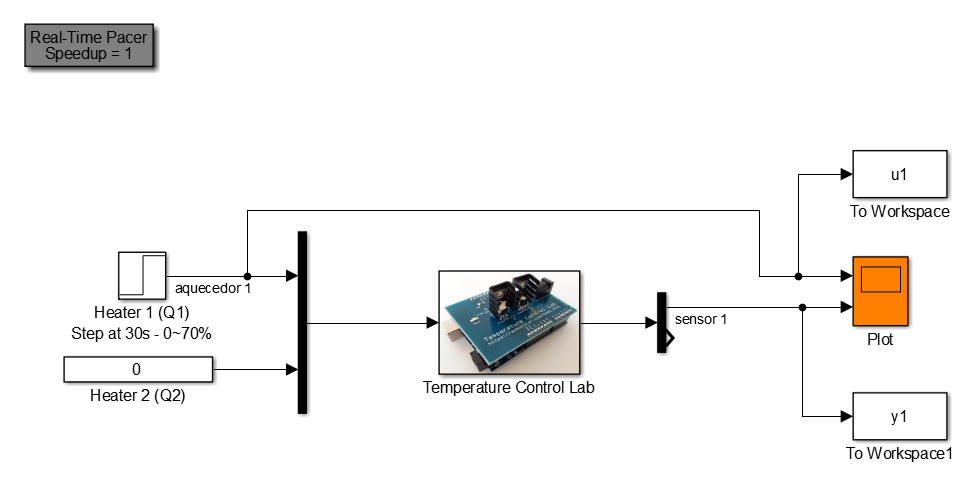
\includegraphics[width=0.9\textwidth]{./5_images/Exp_101_Simulink.png} 
		\label{fig:siso_step_test_simulink}
	\end{center}
    \centering
    \makebox[\width]{Fonte: Autor}
\end{figure}

\begin{figure}
    \caption{Gráfico da coleta de dados SISO}
	\begin{center}
		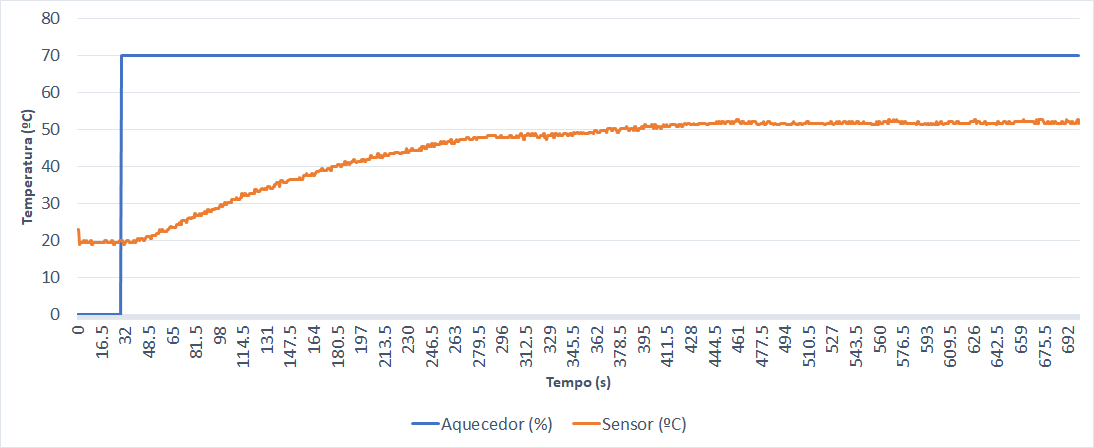
\includegraphics[width=0.9\textwidth]{./5_images/Exp_101_StepTestPlot.png} 
		\label{fig:siso_step_test_plot}
	\end{center}
    \centering
    \makebox[\width]{Fonte: Autor}
\end{figure}

% -----------------------------------------------------------------------------------------------------
% ------------------------------------------- Subsubsection -------------------------------------------
% -----------------------------------------------------------------------------------------------------
\subsubsection{Determinação da estrutura, parâmetros e validação}
\label{subsubsec:siso_identificacao_do_modelo_estrutura}

Através da ferramenta de identificação de sistemas do \acrshort{matlab} foi possível utilizar
os dados obtidos durante a coleta para obtenção de funções de transferência e de representações
através de espaço de estados.

A \cref{fig:siso_systemid_fit} mostra os diferentes modelos testados e indica o Maior Valor do
Fator de Ajuste (FIT) para cada um deles.

A partir dos modelos testados é possível destacar a função de transferência e o modelo de espaço
de estados que apresentam maior FIT e menor ordem. Eles estão indicados nas
\cref{eq:siso_systemid_tf_4p2z} e \cref{eq:siso_systemid_ss_x1} respectivamente.

\begin{figure}
    \caption{Modelos para planta SISO}
	\begin{center}
		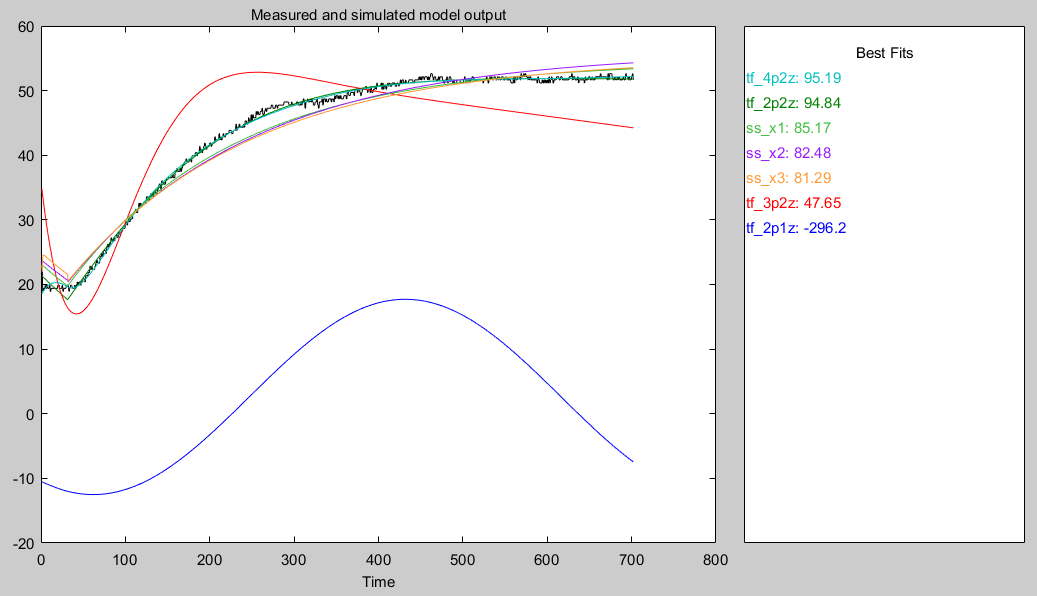
\includegraphics[width=0.9\textwidth]{./5_images/Exp_106_ModelOutput_All.png} 
		\label{fig:siso_systemid_fit}
	\end{center}
    \centering
    \makebox[\width]{Fonte: Autor}
\end{figure}

\begin{equation}
	\label{eq:siso_systemid_tf_4p2z}
    \mathrm{tf\_4p2z} = \dfrac{\\
            3.1952 \mathrm{x10^{-4} s^2} - 7.0930 \mathrm{x10^{-8} s} + 6.7656 \mathrm{x10^{-8}}\\
            }{\\
            \mathrm{s^4} + 6.3814 \mathrm{x10^{-4} s^3} + 1.3026 \mathrm{x10^{-5} s} + 9.0146 \mathrm{x10^{-8}}\\
            }
\end{equation}

\begin{equation}
    \label{eq:siso_systemid_ss_x1}
    \begin{aligned}
        \dfrac{dx}{dt} &= & -5.071 \mathrm{x10^{-3}}\; &x(t) & + 1.069 \mathrm{x10^{-5}}\; &u(t) & + 4.776 \mathrm{x10^{-3}}\; &e(t) \\
        y(t) &= & 369.5\; &x(t) & + 0\; &u(t) & + &e(t)
    \end{aligned}
\end{equation}
\newline

Conforme indicado na \cref{fig:siso_systemid_fit}, o modelo da \cref{eq:siso_systemid_tf_4p2z} apresenta uma
aproximação de 95,19\% e o modelo da \cref{eq:siso_systemid_ss_x1} de 85,17\%.

% .....................................................................................................
% ............................................ Subsection .............................................
% .....................................................................................................
\subsection{Desenvolvimento do controlador}
\label{subsec:siso_desenvolvimento_do_controlador}

A partir do modelo de espaço de estados apresentado na \cref{eq:siso_systemid_ss_x1}, criou-se então
um diagrama de blocos para a parametrização de um controlador \acrshort{mpc} utilizando o
\textit{Model Predictive Control Toolbox} do \acrshort{matlab}.

A \cref{fig:siso_simulink_ss} mostra o diagrama de blocos utilizado para a parametrização do controle
\acrshort{mpc}.

\begin{figure}
    \caption{Diagrama de bloco para parametrização de MPC em planta SISO}
	\begin{center}
		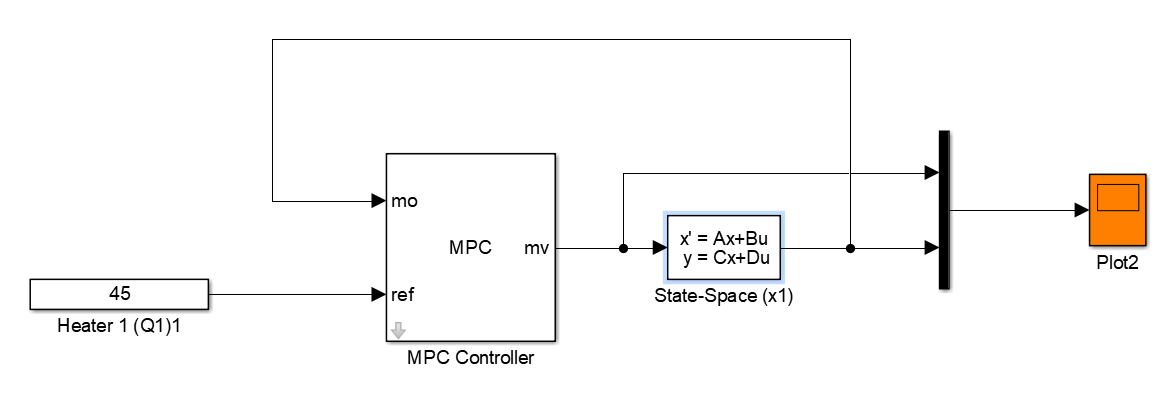
\includegraphics[width=0.9\textwidth]{./5_images/Exp_303_Simulink_SS.png} 
		\label{fig:siso_simulink_ss}
	\end{center}
    \centering
    \makebox[\width]{Fonte: Autor}
\end{figure}

A sintonia do controlador foi baseada tanto na teoria de controle como em resultados experimentais,
sendo que os dados do controlador são detalhados na \cref{tab:mpc_siso_details}.

\begin{table}[h]
	\centering
	\caption{Características do controlador MPC para planta SISO}
	\label{tab:mpc_siso_details}
	\begin{tabular}{lc} \toprule
		{Descrição} 		                            & {Valor}    					\\ \midrule
		Quantidade de estados 		                    & $1$ 						    \\
		Quantidade de entradas 		                    & $1$ 						    \\
		Quantidade de saídas 		                    & $1$ 						    \\
		Quantidade de variáveis manipuladas 		    & $1$ 						    \\
		Quantidade de distúrbios medidos 		        & $0$ 						    \\
		Quantidade de distúrbios não medidos 		    & $0$ 						    \\
		Quantidade de saídas medidas 		            & $1$ 						    \\
		Tempo de amostragem 		                    & $1$ segundo 					\\
		Horizonte de predição 		                    & $100$  						\\
		Horizonte de controle 		                    & $15$  						\\
		Peso: Variáveis Manipuladas 		            & $0$  						    \\
		Peso: Taxa de Variáveis Manipuladas 		    & $0.0619$  				    \\
		Peso: Variáveis de Saída 		                & $1.6161$  					\\
		Peso: ECR 		                                & $100000$  					\\
		Estimador de Estados 		                    & Filtro de Kalman padrão  		\\
		Limitantes: Entrada 		                    & Entre $0$ e $100\%$  			\\ \bottomrule
	\end{tabular}
	\caption*{Fonte: Autor}
\end{table}

% .....................................................................................................
% ............................................ Subsection .............................................
% .....................................................................................................
\subsection{Aplicação do controlador MPC na planta SISO}
\label{subsec:siso_mpc_and_plant}

Através do controlador descrito na \cref{tab:mpc_siso_details} pode-se então desenvolver um diagrama
de blocos para a implementação do controle na planta \acrshort{tclab}. O diagrama de blocos é
apresentado na \cref{fig:siso_simulink_mpc_and_plant}.

\begin{figure}
    \caption{Diagrama de bloco para aplicação de MPC em planta SISO}
	\begin{center}
		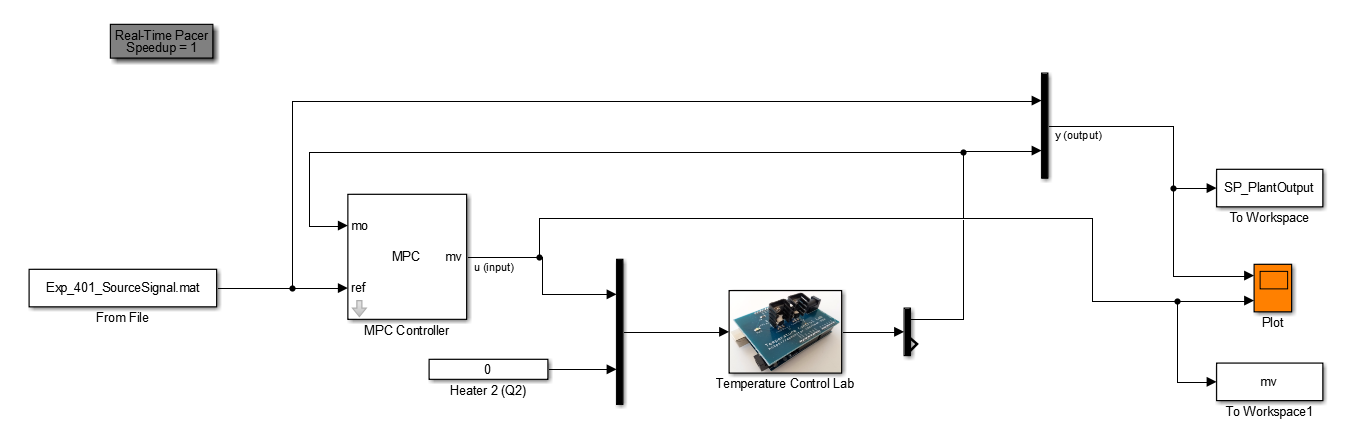
\includegraphics[width=0.9\textwidth]{./5_images/Exp_402_Simulink.png} 
		\label{fig:siso_simulink_mpc_and_plant}
	\end{center}
    \centering
    \makebox[\width]{Fonte: Autor}
\end{figure}

O resultado da aplicação do controlador conforme o diagrama de blocos da \cref{fig:siso_simulink_mpc_and_plant}
pode ser verificado nos gráficos presentes das \crefrange{fig:siso_mpc_and_plant_plot01}{fig:siso_mpc_and_plant_plot03}.

\begin{figure}
    \caption{MPC em planta SISO - \textit{Setpoint} e Valor medido}
	\begin{center}
		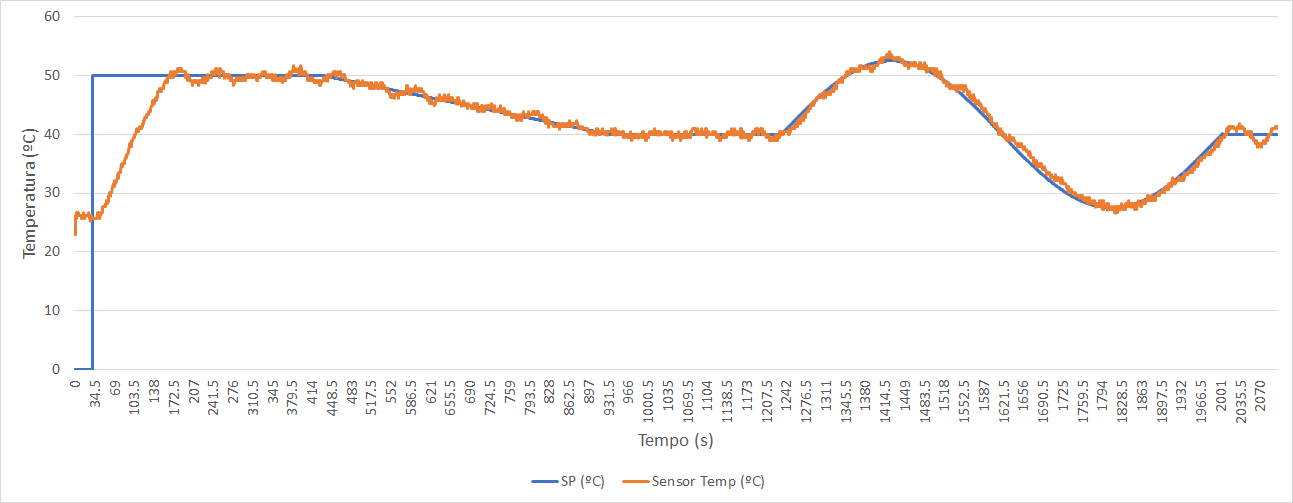
\includegraphics[width=0.9\textwidth]{./5_images/Exp_401_PlotResults_01_SS_x1_6.png} 
		\label{fig:siso_mpc_and_plant_plot01}
	\end{center}
    \centering
    \makebox[\width]{Fonte: Autor}
\end{figure}

\begin{figure}
    \caption{MPC em planta SISO - Potência do aquecedor de entrada}
	\begin{center}
		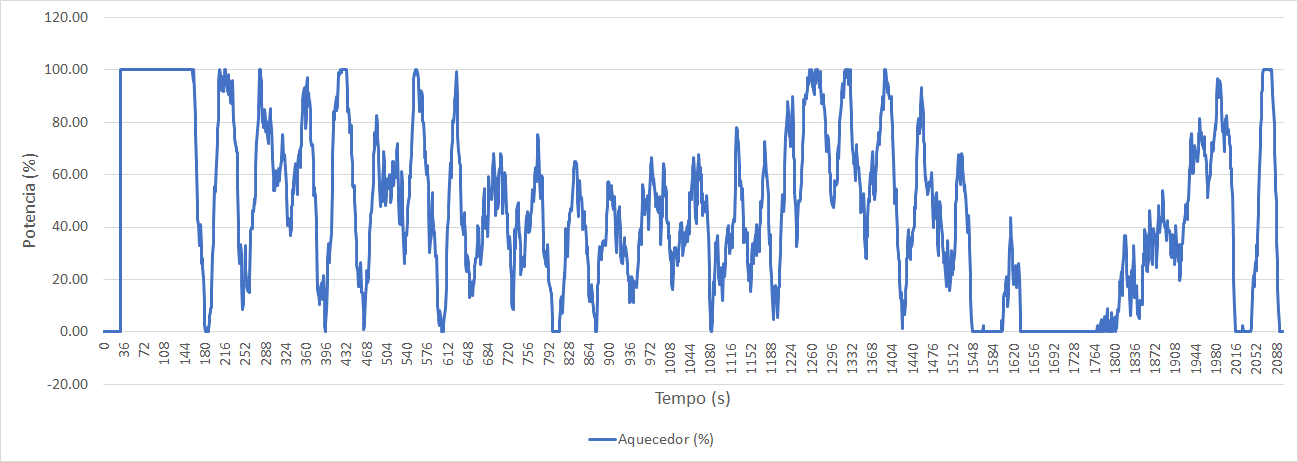
\includegraphics[width=0.9\textwidth]{./5_images/Exp_401_PlotResults_02_SS_x1_6.png} 
		\label{fig:siso_mpc_and_plant_plot02}
	\end{center}
    \centering
    \makebox[\width]{Fonte: Autor}
\end{figure}

\begin{figure}
    \caption{MPC em planta SISO - Erro calculado}
	\begin{center}
		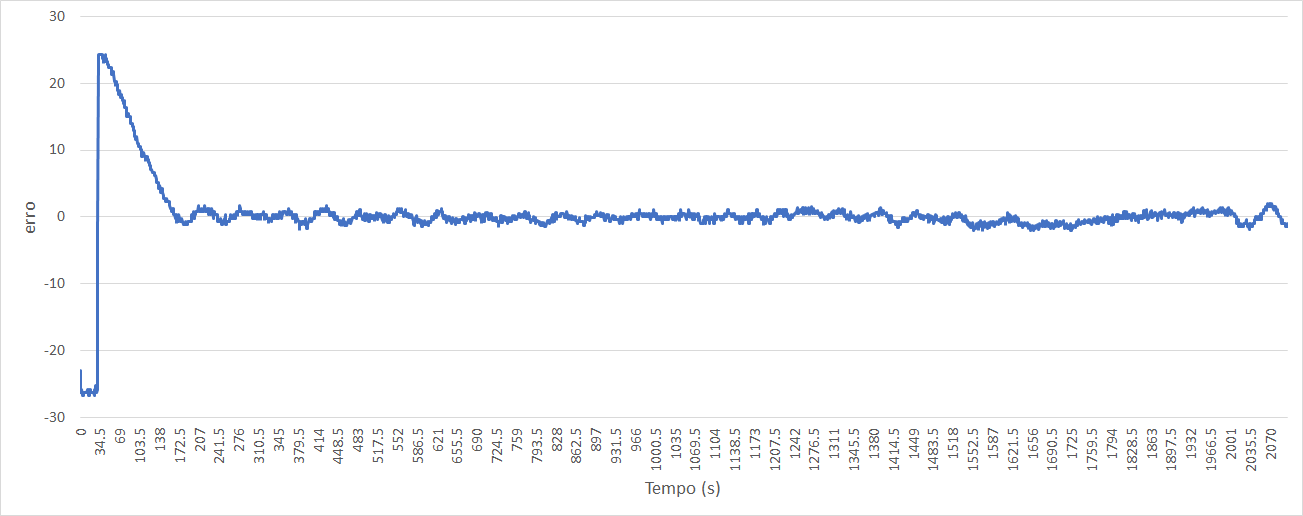
\includegraphics[width=0.9\textwidth]{./5_images/Exp_401_PlotResults_03_SS_x1_6.png} 
		\label{fig:siso_mpc_and_plant_plot03}
	\end{center}
    \centering
    \makebox[\width]{Fonte: Autor}
\end{figure}